\documentclass[aspectratio=169,ignorenonframetext]{beamer}


\usepackage[english]{babel}
\usepackage[T1]{fontenc}
\usepackage{harveyballs}
\usepackage[super]{nth}
\usepackage{graphicx}
\usepackage{tikz}
\usepackage{todonotes}
\usepackage{multicol}
\usepackage{minted}
\usepackage{txfonts}


\usemintedstyle{colorful}
\usetikzlibrary{shapes,arrows}


\newcommand\term[1]{{\bf #1}}
\newcommand\enumlabel[1]{{\bf\emph{#1}}}
\newcommand\donenone\harveyBallNone{}
\newcommand\donehalf\harveyBallHalf{}
\newcommand\donefull\harveyBallFull{}


\usetheme{simspace}
\setbeamercovered{transparent}
\AtBeginSection{\frame{\sectionpage}}


\title[Haskell: What To Do When Success Can't Be Avoided]
{Haskell: What To Do When Success Can't Be Avoided}

\author{Sukant Hajra}
\institute{Haskell eXchange 2021}
\day=17\relax
\month=11\relax
\year=2021\relax

\begin{document}

\maketitle

\begin{frame}
	\titlepage{}
\end{frame}

\section{SimSpace and Me}

\begin{frame}{Hi!}
	\begin{columns}
		\column{.5\textwidth}
		{\tt
			Sukant Hajra \\
			@shajra \\
			sukant@simspace.com
		}
		\column{.5\textwidth}
		\begin{itemize}
			\item FP and Haskell enthusiast
			\item SimSpace Manager
			\item SimSpace Recruiter
		\end{itemize}
	\end{columns}
	\begin{exampleblock}{}
		We're hiring!
	\end{exampleblock}
\end{frame}

\begin{frame}{Contributed ideas}
	\begin{multicols}{3}
		Alec Heller \\
		Alex Sturtz \\
		Cary Robbins \\
		Cullin Poresky \\
		Dan Fithian \\
		Daniel Bergey \\
		David Dvorak \\
		Devin Lehmacher \\
		Jason Shipman \\
		Jeff Dwyer \\
		Matt Russell \\
		Mike Beynon \\
		Nicolas Hery \\
		Paul Gray \\
		Rick Owens \\
		Samuel Schlesinger \\
		Scott Fleischman \\
		Stuart Terrett \\
		Travis Staton \\
		William Yao
	\end{multicols}
\end{frame}

\begin{frame}{SimSpace's product}
	\begin{multicols}{2}
		\begin{itemize}
			\item simulate production networks
			      \begin{itemize}
				      \item specification of ranges
				      \item deployment of ranges
			      \end{itemize}
			\item live events
			      \begin{itemize}
				      \item tracking
				      \item scoring
			      \end{itemize}
			      \columnbreak
			\item automation
			      \begin{itemize}
				      \item attacks
				      \item user emulation
				      \item defense
				      \item scoring
			      \end{itemize}
			\item learning management for training
			\item workforce management
			\item risk assessment
		\end{itemize}
	\end{multicols}
\end{frame}

\begin{frame}{SimSpace Portal: Attacks}
	\begin{center}
		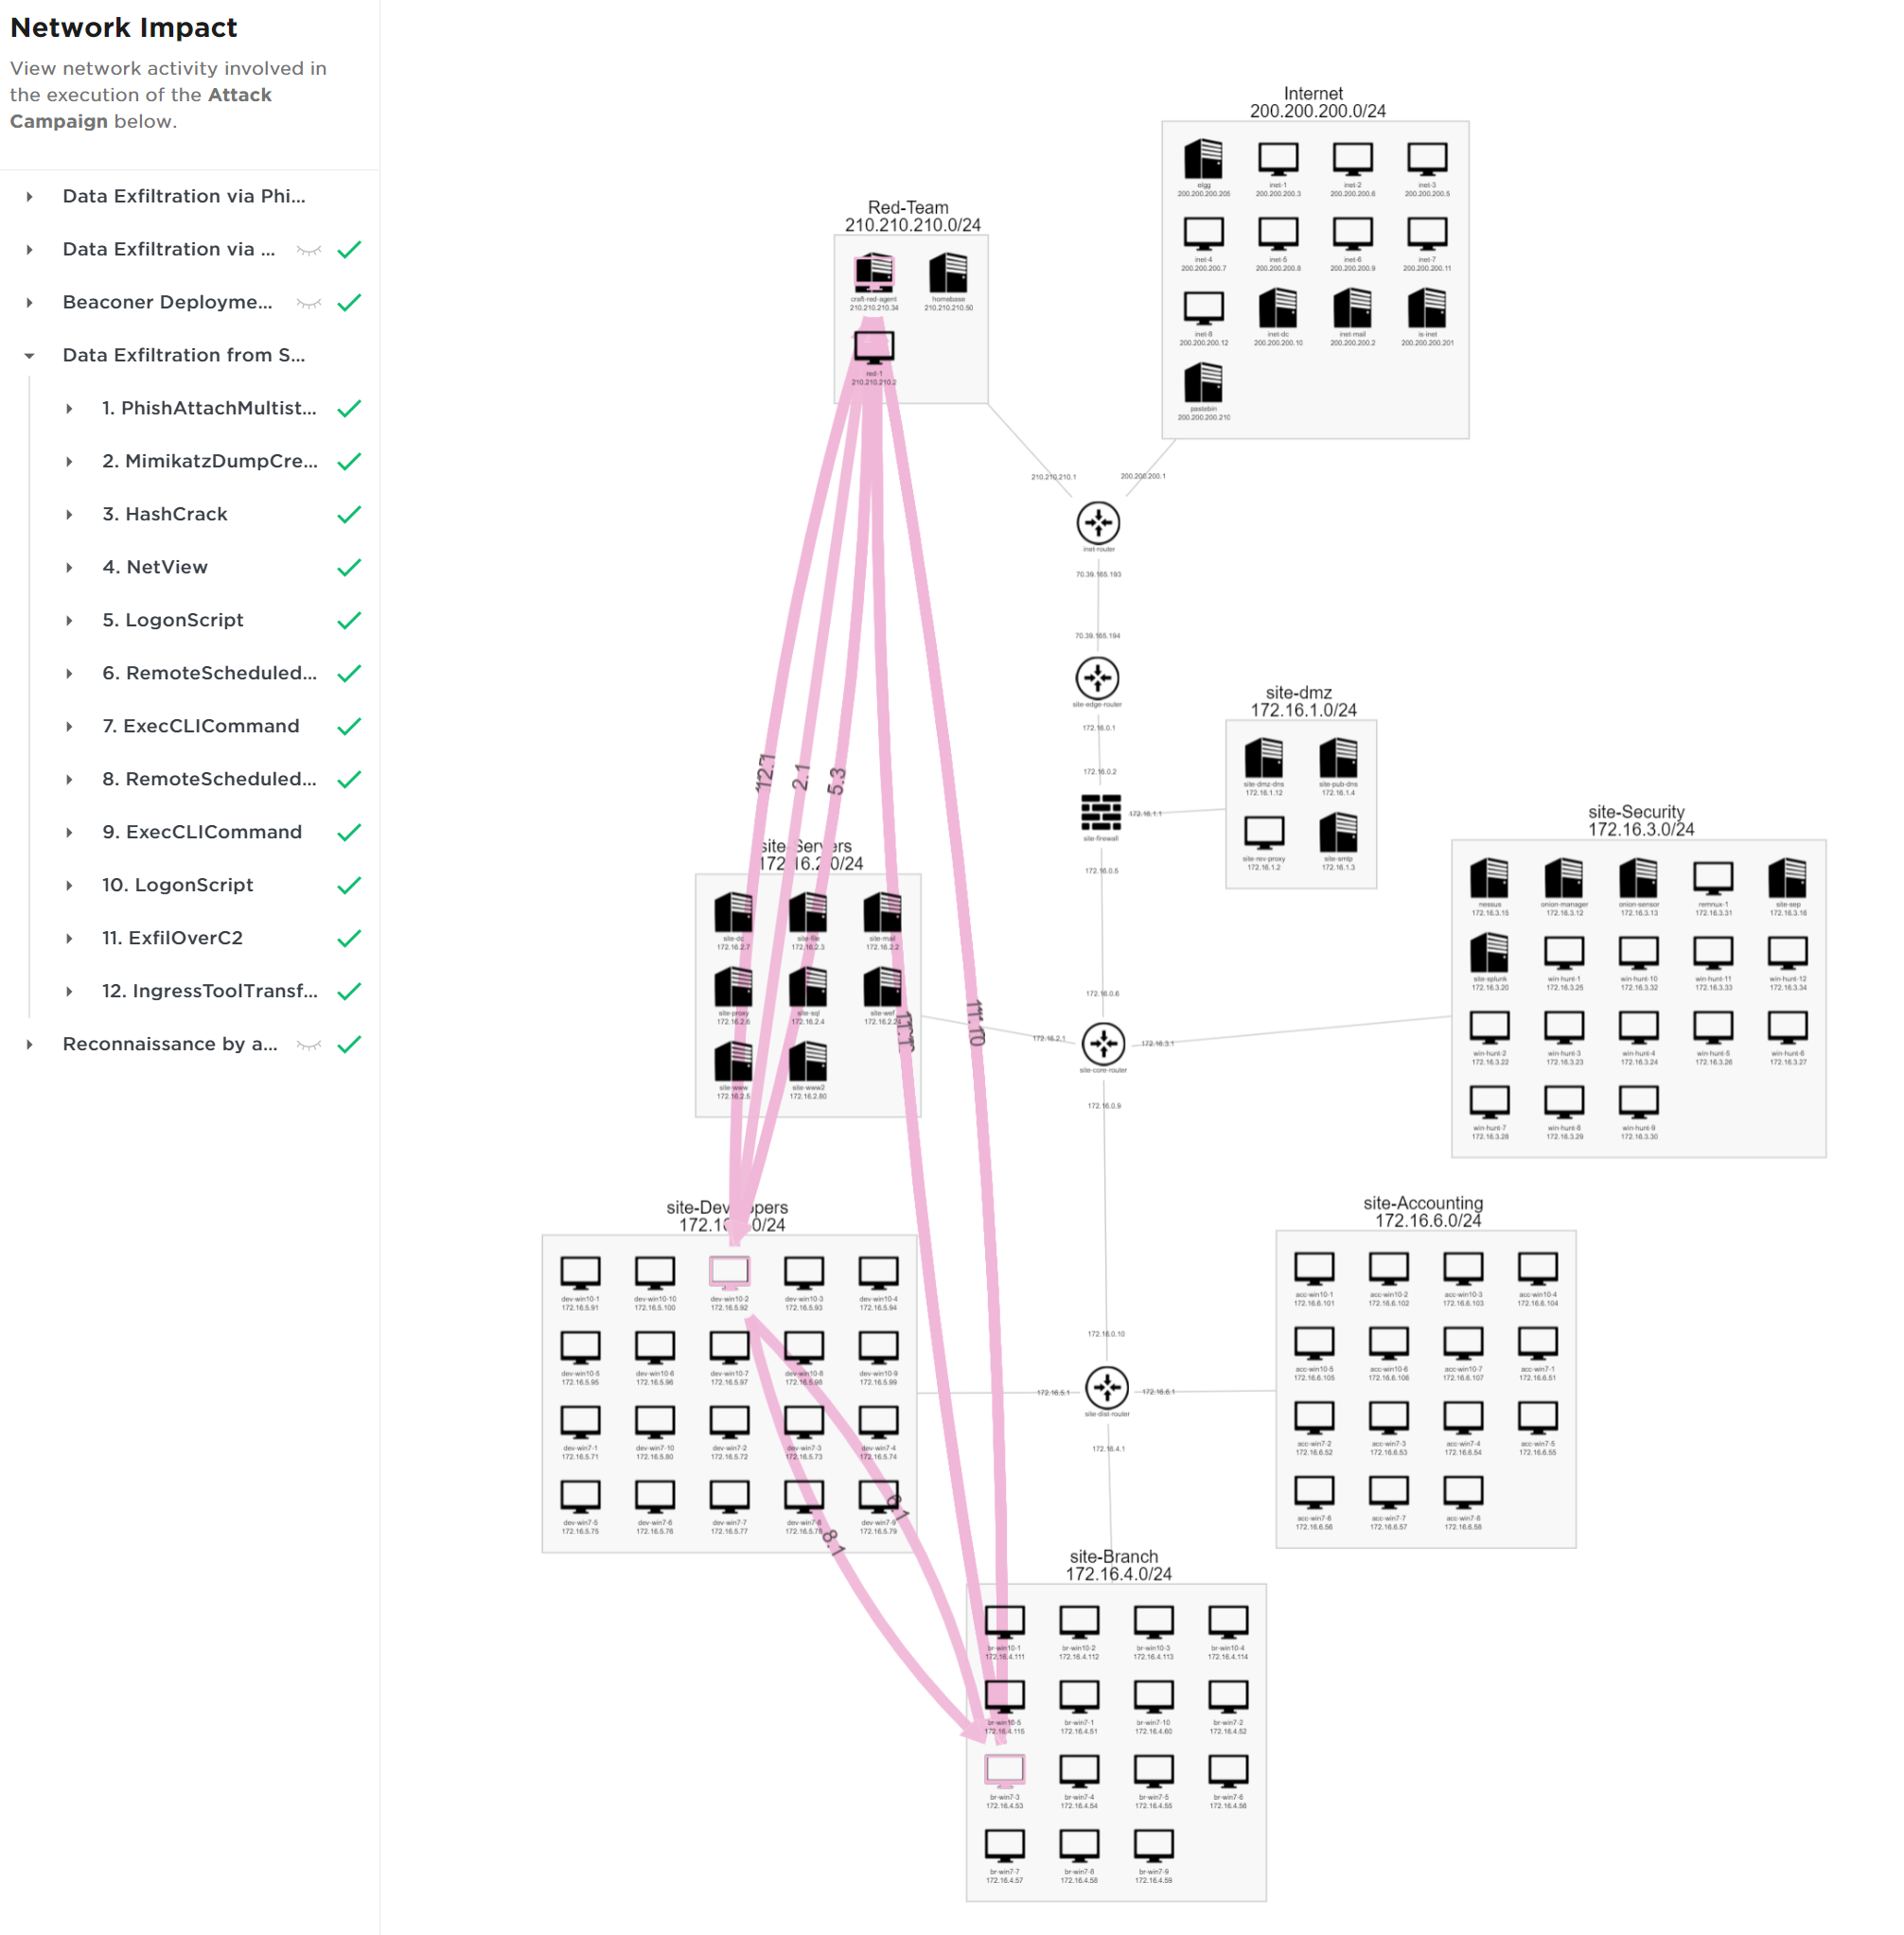
\includegraphics[height=.6\textheight]{images/automated_attacks.png}
	\end{center}
\end{frame}

\begin{frame}{SimSpace Portal: Scoring}
	\begin{center}
		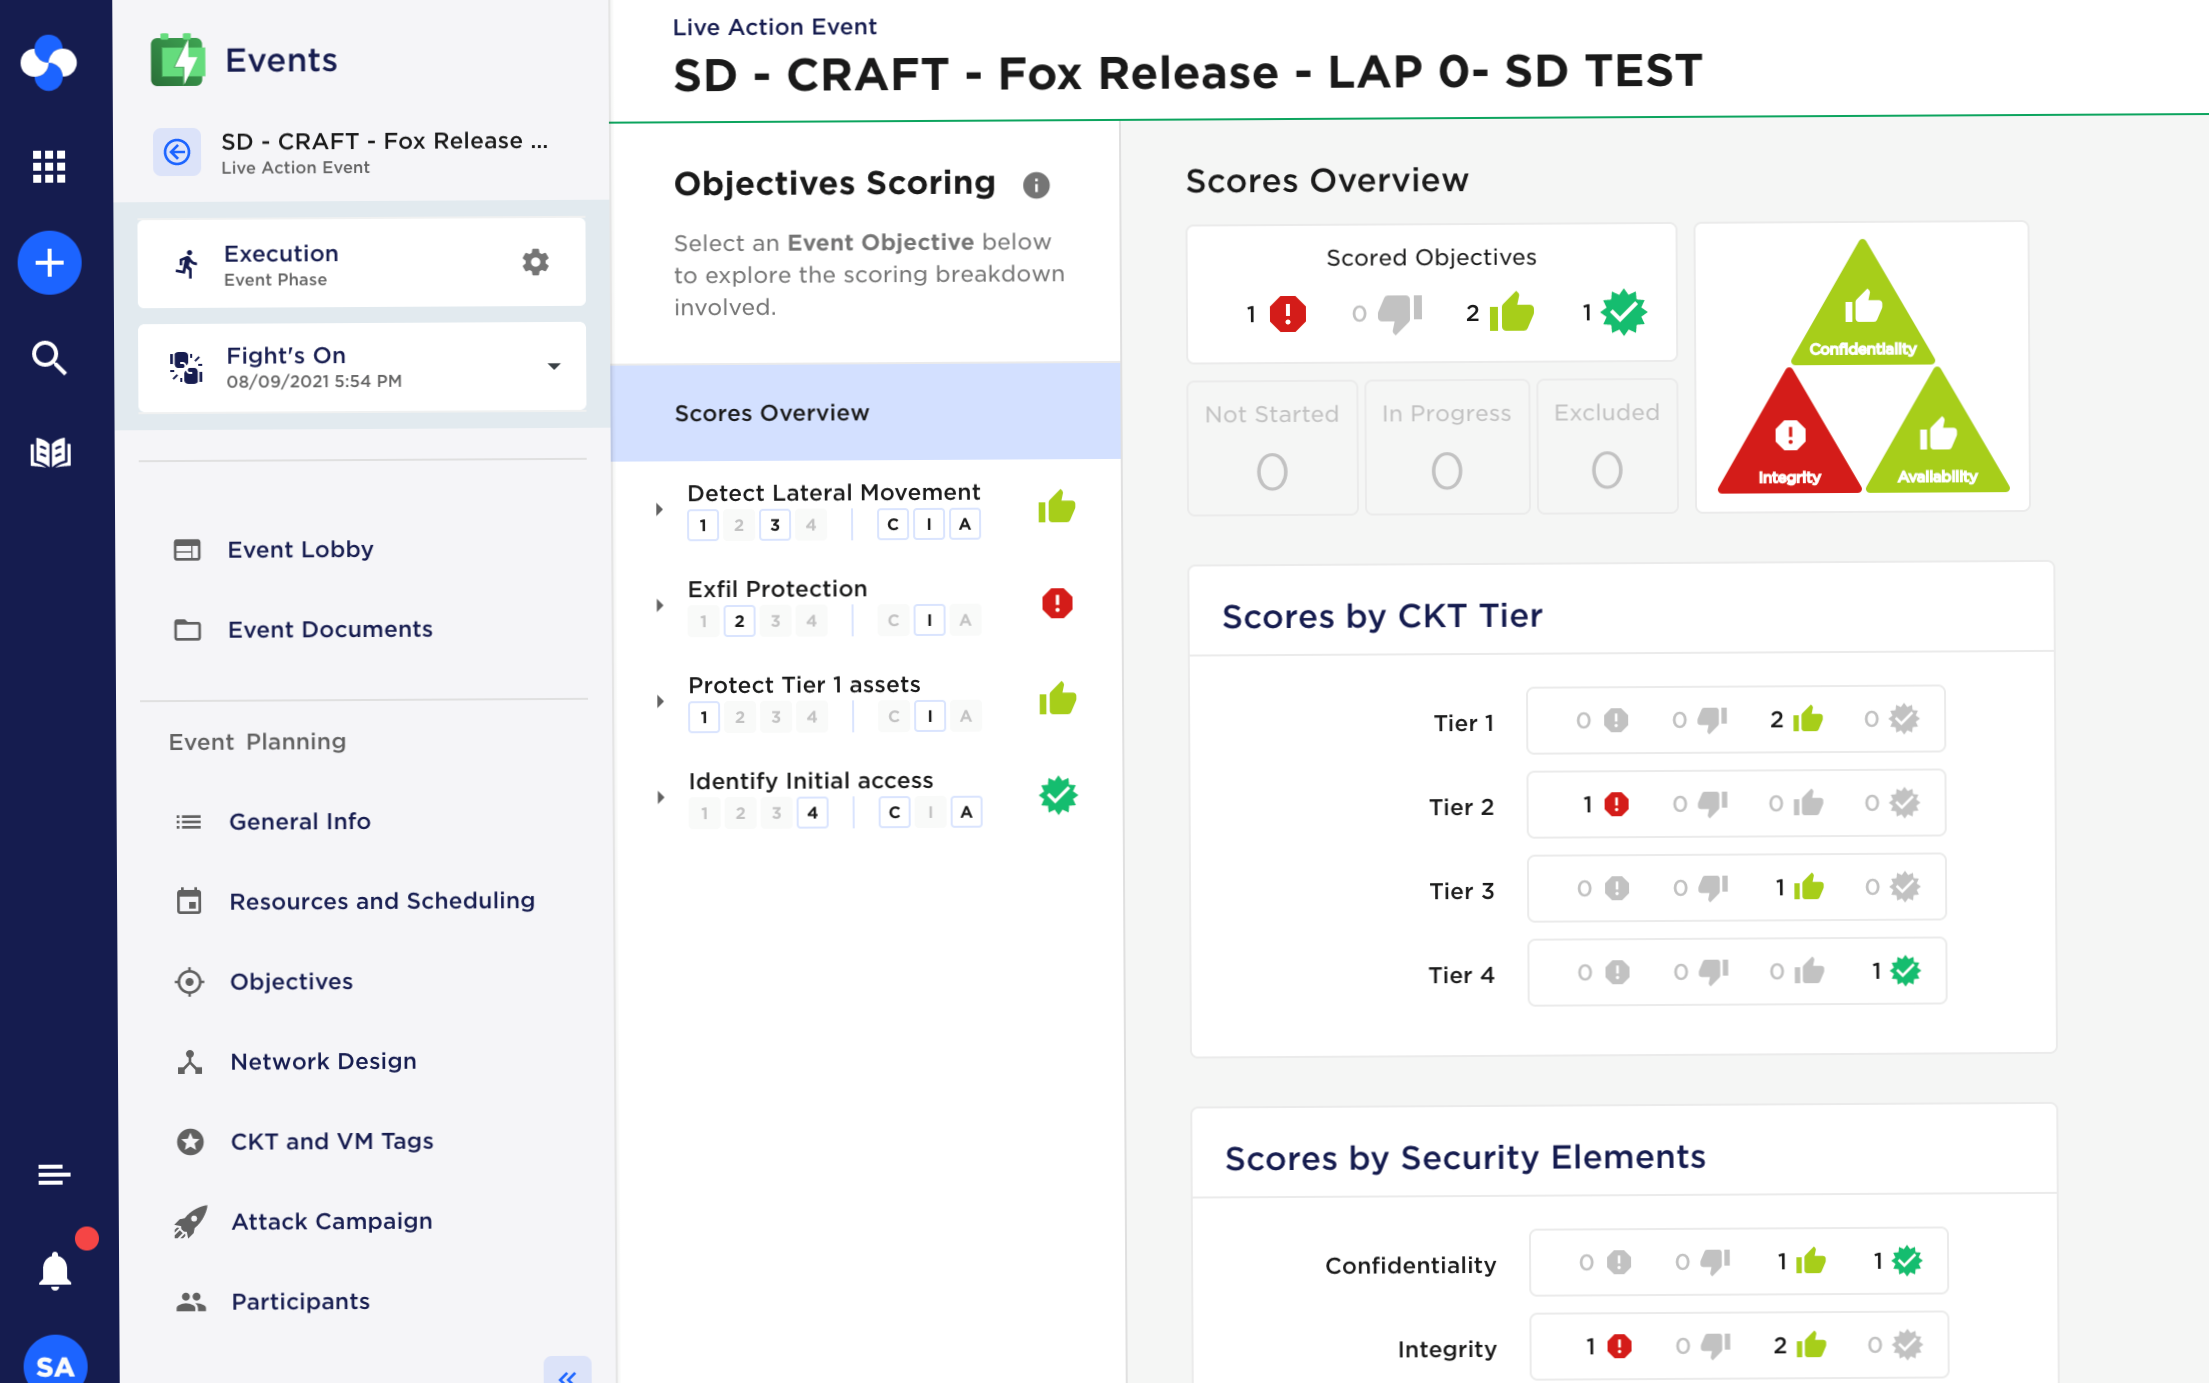
\includegraphics[height=.6\textheight]{images/objective_scoring.png}
	\end{center}
\end{frame}

\begin{frame}{SimSpace Portal: Learning modules}
	\begin{center}
		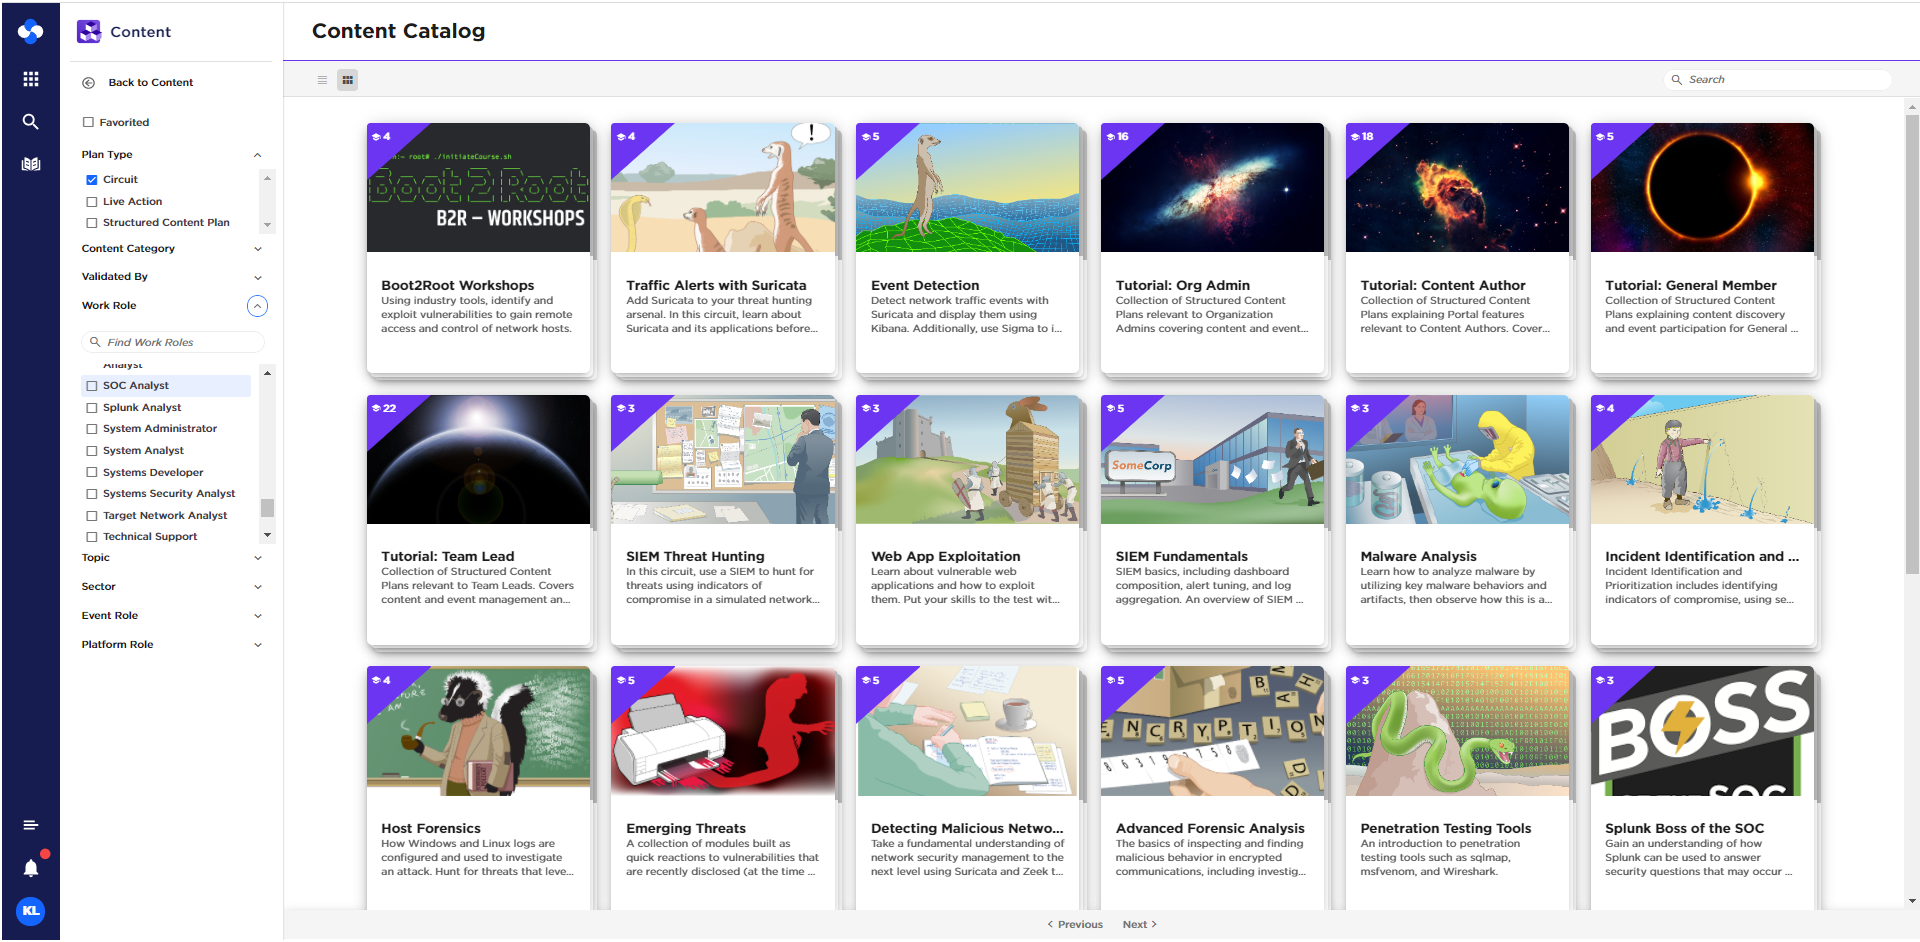
\includegraphics[height=.6\textheight]{images/learning_paths.png}
	\end{center}
\end{frame}

\begin{frame}{Architectural sketch}
	\begin{center}
		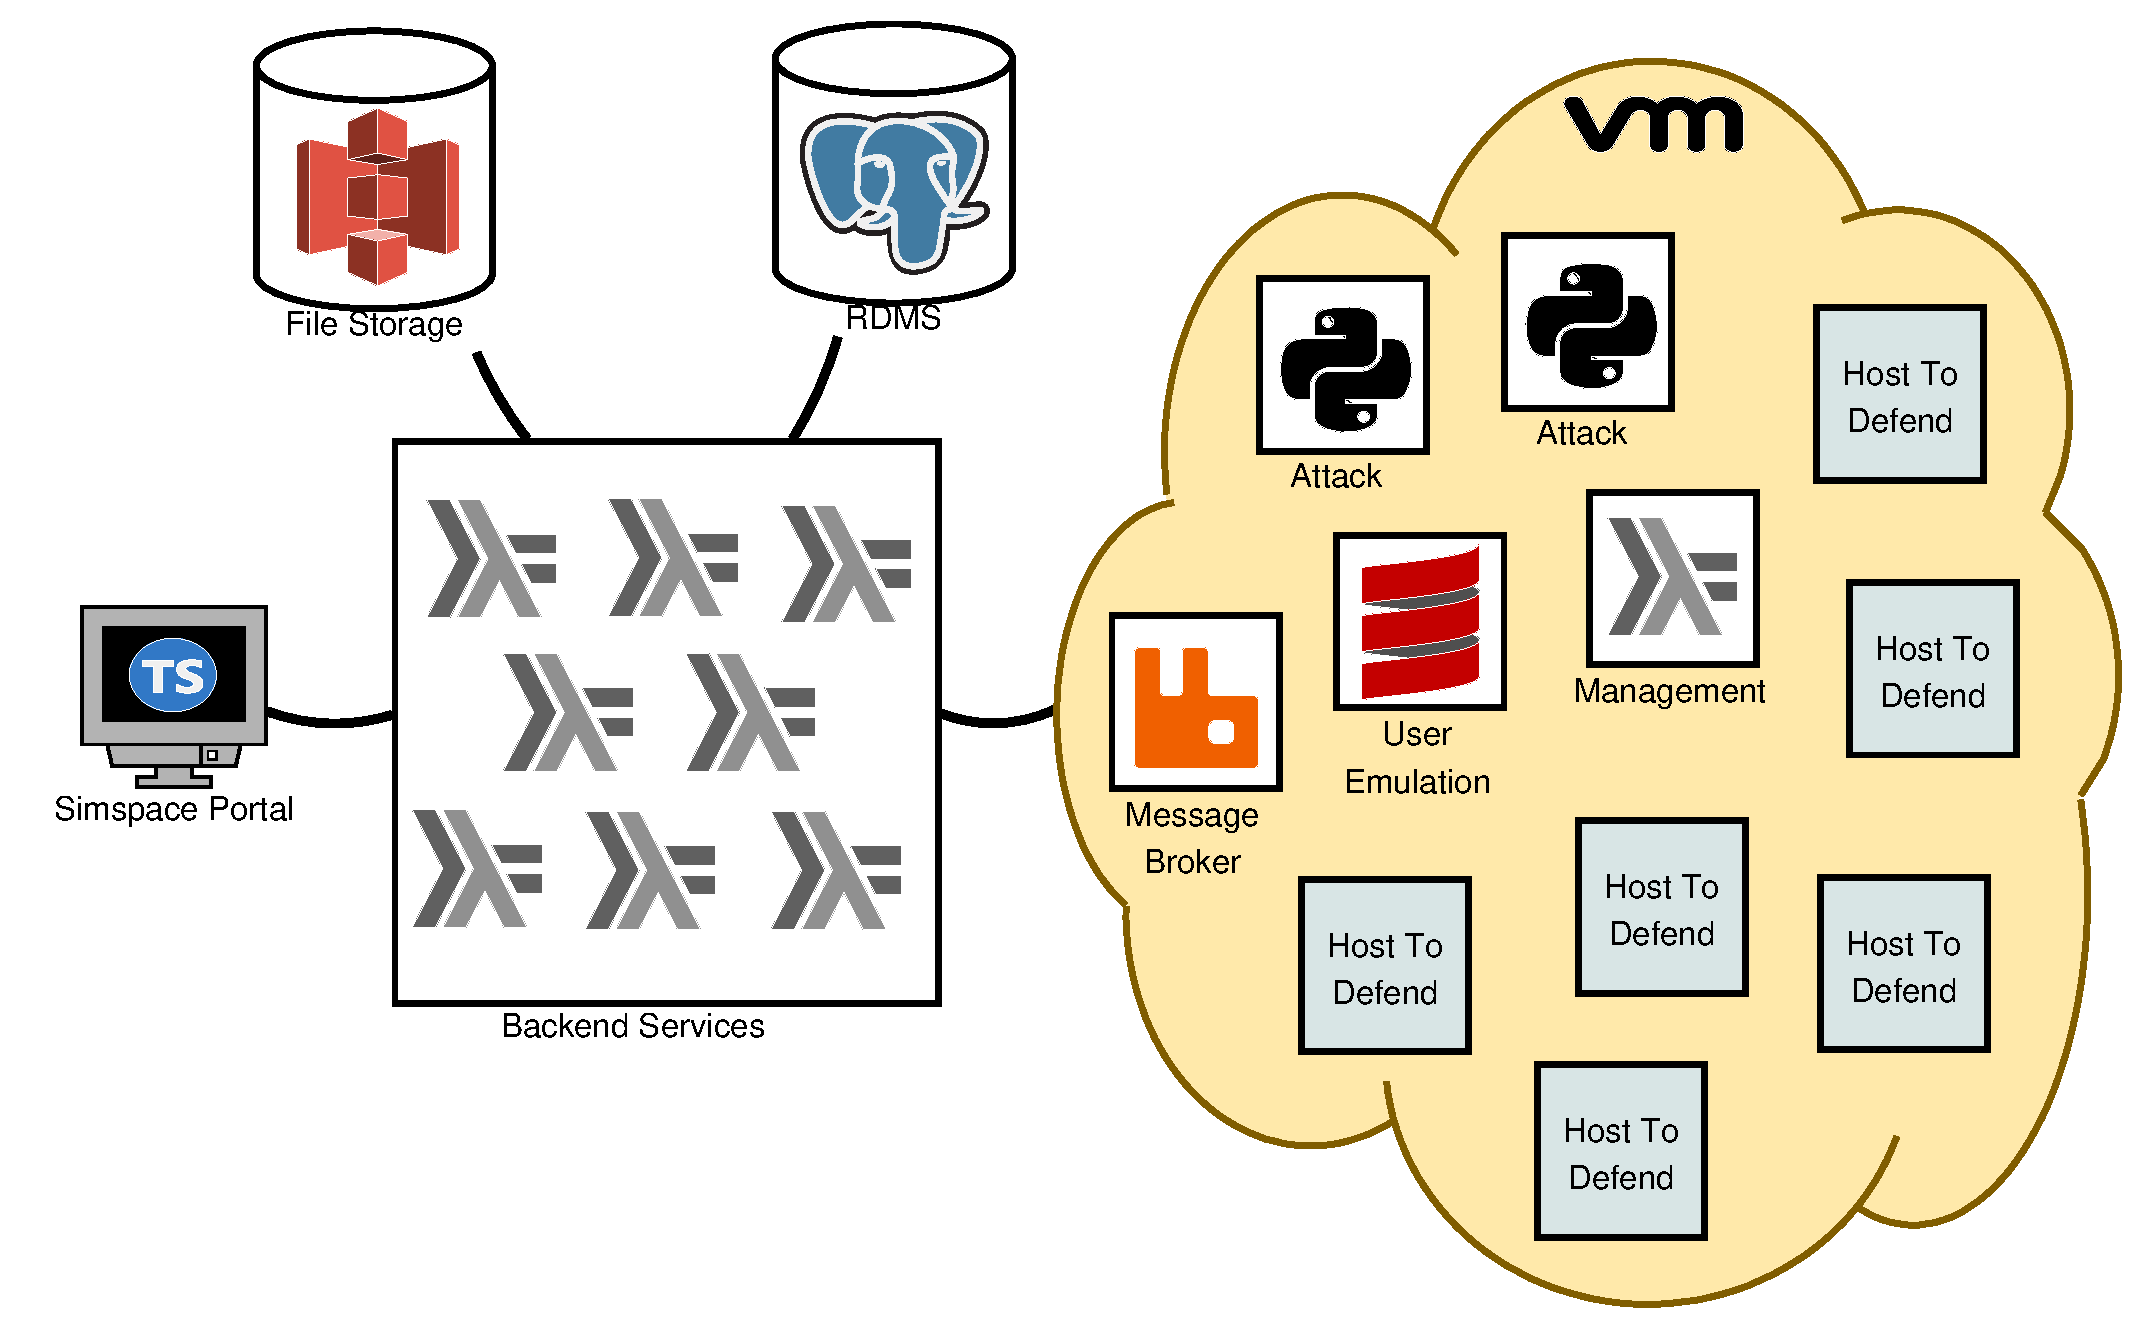
\includegraphics[height=.6\textheight]{images/portal.eps}
	\end{center}
\end{frame}

\begin{frame}{Haskell isn't everywhere}
	\begin{columns}
		\column{.5\textwidth}
		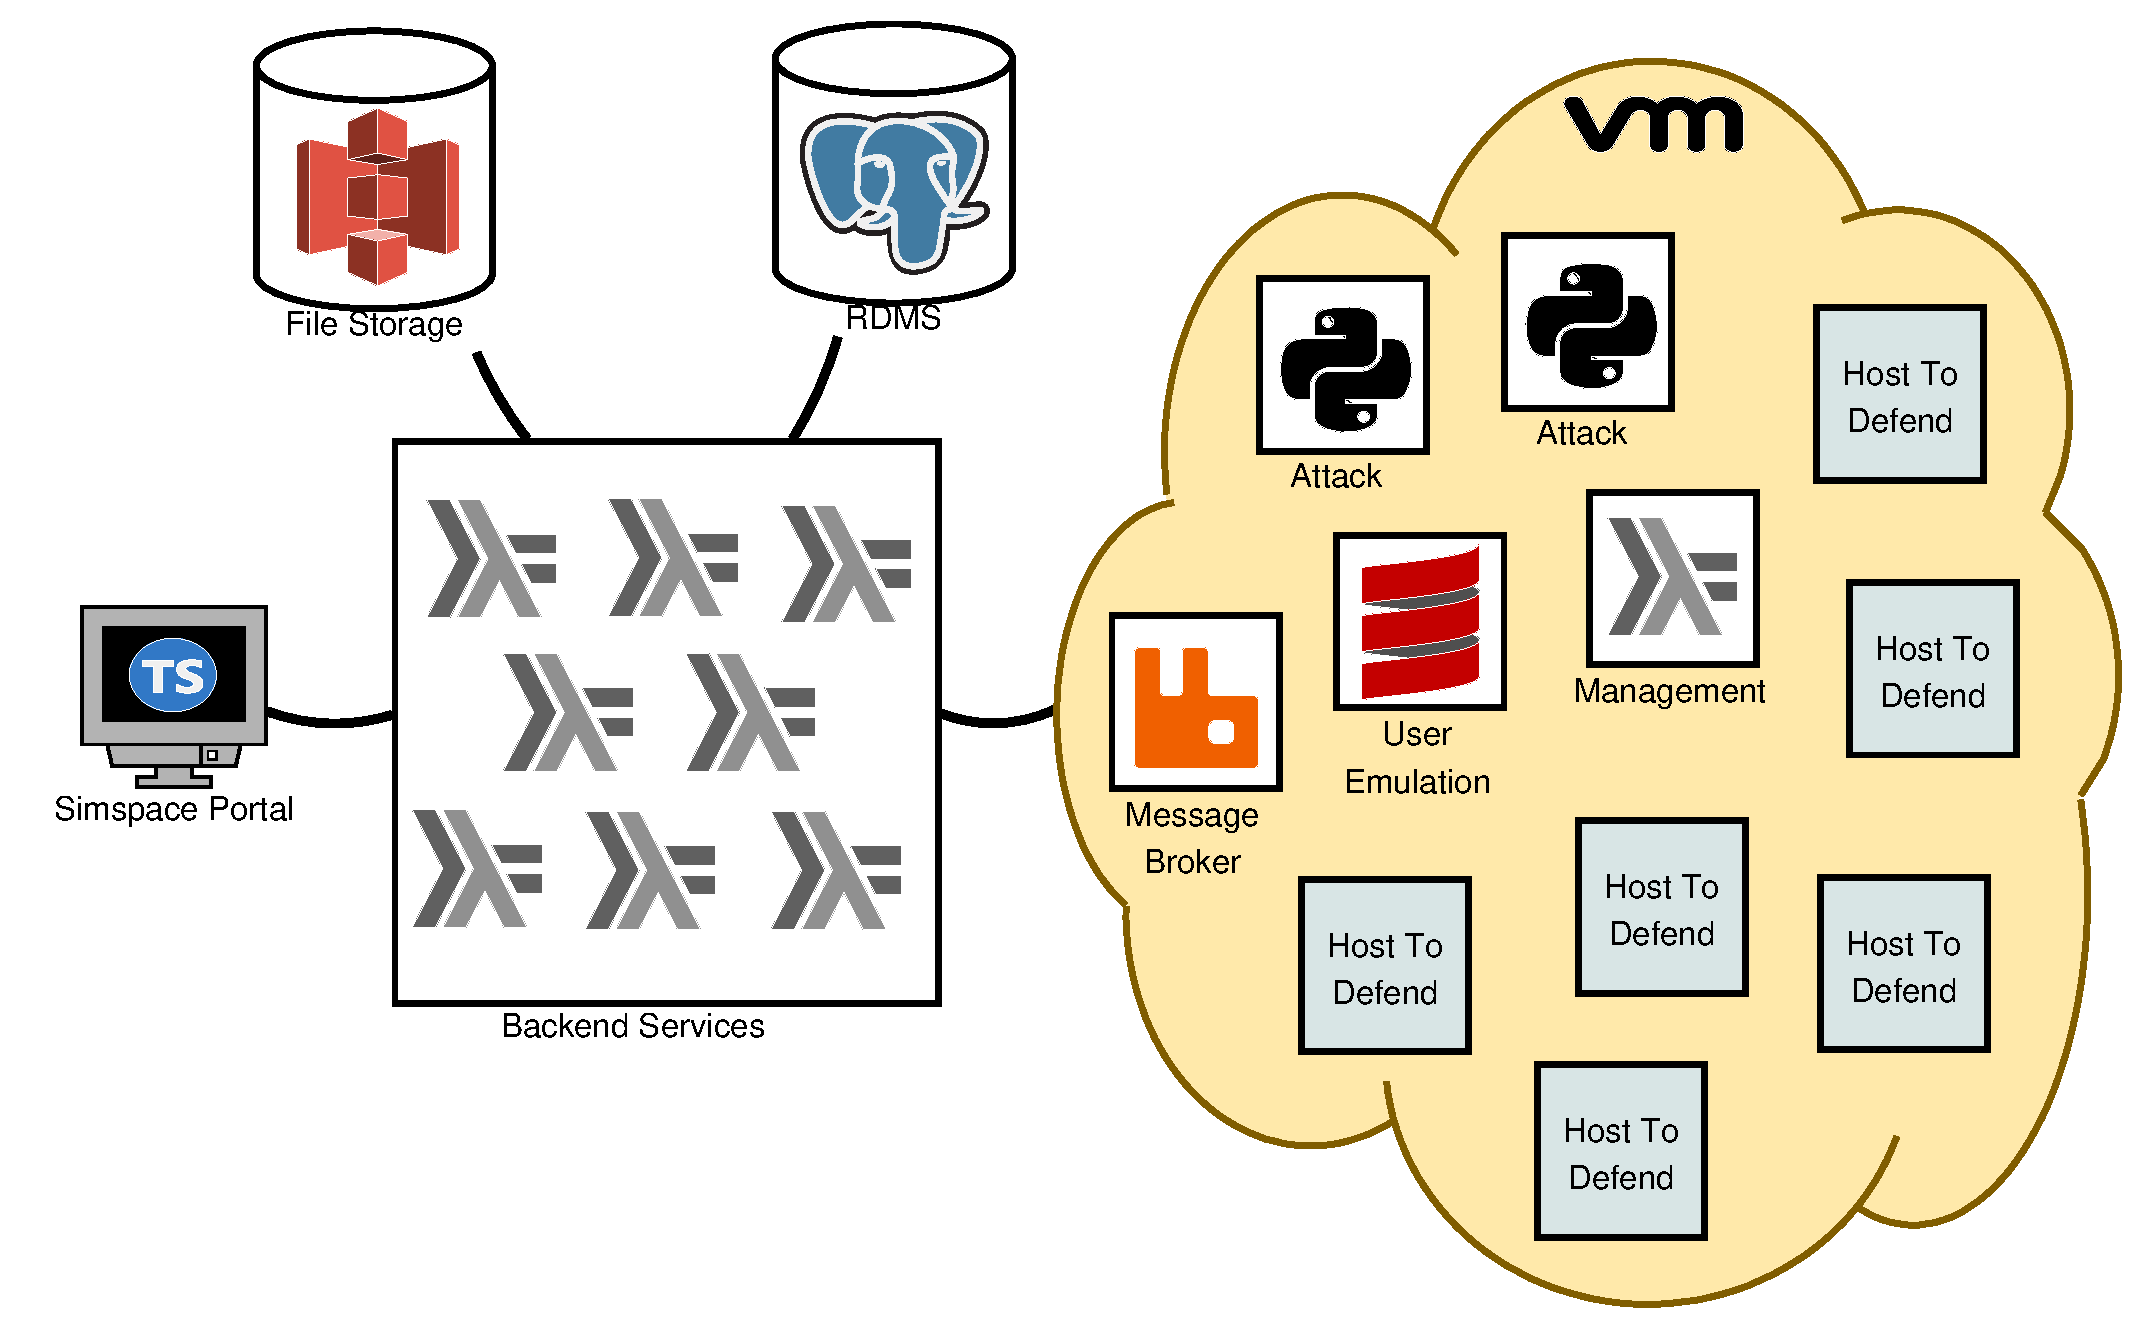
\includegraphics[width=\textwidth]{images/portal.eps}
		\column{.5\textwidth}
		\begin{exampleblock}{}
			Respect the expertise of other domains.
		\end{exampleblock}
		\begin{exampleblock}{}
			Evaluate Haskell's limitations honestly.
		\end{exampleblock}
	\end{columns}
\end{frame}

\begin{frame}{Some statistics}
	\begin{columns}
		\column{.5\textwidth}
		\begin{block}{Employees}
			\begin{itemize}
				\item $\sim$250 employees total
				\item 10 Design/UX
				\item 25 Frontend
				\item 8 QA
				\item 33 Backend (Haskell)
			\end{itemize}
		\end{block}
		\column{.5\textwidth}
		\begin{block}{Engineering Teams}
			\begin{itemize}
				\item 8 feature teams
				\item 1 team focused on scaling
				\item 1 team focused on internal tools
			\end{itemize}
		\end{block}
		\begin{block}{Code}
			$\sim$441,000 lines of Haskell
		\end{block}
	\end{columns}
\end{frame}

\section{Branding and Perception}

\begin{frame}{Haskell's brand}
	\begin{columns}
		\column{.5\textwidth}
		Evolution of Haskell's branding:
		\begin{itemize}
			\item<1-> ``(Avoid success) at all costs.''
			\item<2-> ``Avoid (success at all costs).''
			\item<2-> ``Avoid (success at any cost).''
			\item<2-> ``Have success at a fair cost.''
		\end{itemize}
		\column{.5\textwidth}
		\begin{exampleblock}<3->{}
			Your brand is now related to Haskell's brand.
		\end{exampleblock}
		\begin{exampleblock}<3->{}
			Give room for Haskell to innovate.
			\begin{itemize}
				\item Budget time for updates.
				\item Keep up with updates.
			\end{itemize}
		\end{exampleblock}
	\end{columns}
\end{frame}

\begin{frame}{Academia's brand}
	\begin{columns}
		\column{.45\textwidth}
		From the 2010 Edsger W. Dijkstra Memorial Lecture at UT Austin
		\begin{itemize}
			\item 7 ways to differentiate scientists from engineers:
			      \begin{multicols}{2}
				      \begin{itemize}
					      \item Timescale
					      \item Idealism
					      \item Certainty
					      \item Generality
					      \item Separation of concerns
					      \item Originality
					      \item Formalization
				      \end{itemize}
			      \end{multicols}
			\item We need \emph{synthesis} of both.
		\end{itemize}
		\column{.55\textwidth}
		\begin{exampleblock}<2->{}
			We need an updated model for scientists and engineers.
		\end{exampleblock}
		\begin{exampleblock}<2->{}
			Synthesis between science and engineering should be accessible, even commonplace.
		\end{exampleblock}
		\begin{exampleblock}<2->{}
			We need more stories from industry of synthesis.
		\end{exampleblock}
		\begin{exampleblock}<2->{}
			We are stewards of academia's brand.
		\end{exampleblock}
	\end{columns}
\end{frame}

\section{Synthesis: Avaleryar}

\begin{frame}{Motivation for Avaleryar}
	Authorization is hard
	\begin{itemize}
		\item Persnickety, ad hoc logic distributed across the code
		\item Simple models (ACLs, RBAC, etc.) require complex interpretations
		\item Awkward coupling with business logic
	\end{itemize}
\end{frame}

\begin{frame}{Logic programming!}
	In their paper on \emph{Soutei}, Pimlott and Kiselyov describe a datalog variant:
	\begin{itemize}
		\item The application provides facts about the requested action (axioms)
		\item policies specify the derivation of other facts (inferences rules)
		\item the authorization system is a policy compliance checker [\ldots]
		\item the compliance checker is a deduction engine.
	\end{itemize}

	\begin{block}{SimSpace's implementation}
		\url{https://github.com/SimSpace/avaleryar}
	\end{block}
\end{frame}

\begin{frame}[fragile]{Avaleryar policy example}
	\begin{columns}
		\column{.45\textwidth}
		\begin{block}{}
			\begin{verbatim}
can(?activity) :-
  want-to(?activity).

can(sing).

;; we can dance if we want to
want-to(dance).

;; we can act if we want to
want-to(act).
		    \end{verbatim}
		\end{block}
		\column{.55\textwidth}
		\begin{block}{}
			\begin{verbatim}
;; we only want to go when the
;; night is young, and so am I
want-to(go) :-
  clock says time-of(night, young),
  bio says age-of(me, young).
		    \end{verbatim}
		\end{block}
	\end{columns}
\end{frame}

\begin{frame}[fragile]{Avaleryar policy example}
	\begin{block}{}
		\begin{verbatim}
;; we can overextend the efficacy of
;; a questionable pop-culture reference
safety(?activity) :-
  can(?activity),
  application says out-of(control, everything),
  application says doing-it(from, pole),
  application says doing-it(to, pole),
  application says looking-at(hands, ?somebody),
  ?somebody says taking(the-chance).
		\end{verbatim}
	\end{block}
\end{frame}

\begin{frame}[fragile]{Avaleryar library usage}
	\begin{block}{}
		\begin{minted}{haskell}
class Factual a where
  toFact :: a -> Fact

establishSafety :: Handle -> Activity -> IO (Either Error Bool)
establishSafety hdl activity =
    checkQuery hdl facts "safety" [val activity]
  where facts = [ toFact $ OutOf Control Everything
                , toFact $ DoingIt FromPole
                , toFact $ DoingIt ToPole
                , toFact $ LookingAtHands "jenny" ]
        \end{minted}
	\end{block}
\end{frame}

\begin{frame}{Avaleryar takeaways}
	\begin{columns}
		\column{.5\textwidth}
		\begin{exampleblock}{}
			Haskell is great for implementing languages.
		\end{exampleblock}
		\column{.5\textwidth}
		\begin{exampleblock}{}
			It's worth finding a way to integrate academic and non-academic
			employees.
		\end{exampleblock}
	\end{columns}
\end{frame}

\section{Synthesis: Servant}

\begin{frame}[fragile]{Type-level DSL}
	\begin{block}{Haskell-side specification: \tt{GET notifications/meta}}
		\begin{minted}{haskell}
data NotificationSubscriberRoutes route = NotificationSubscriberRoutes
  { getNotificationsMeta :: route :-
      "notifications"
        :> "meta"
        :> Get '[SIMJSON] Core.MetaResponse
    ...
  } deriving stock (Generic)
        \end{minted}
	\end{block}
	With Servant, we get an HTTP client for low-cost.
\end{frame}

\begin{frame}{More type-level payoff}
	\begin{figure}
		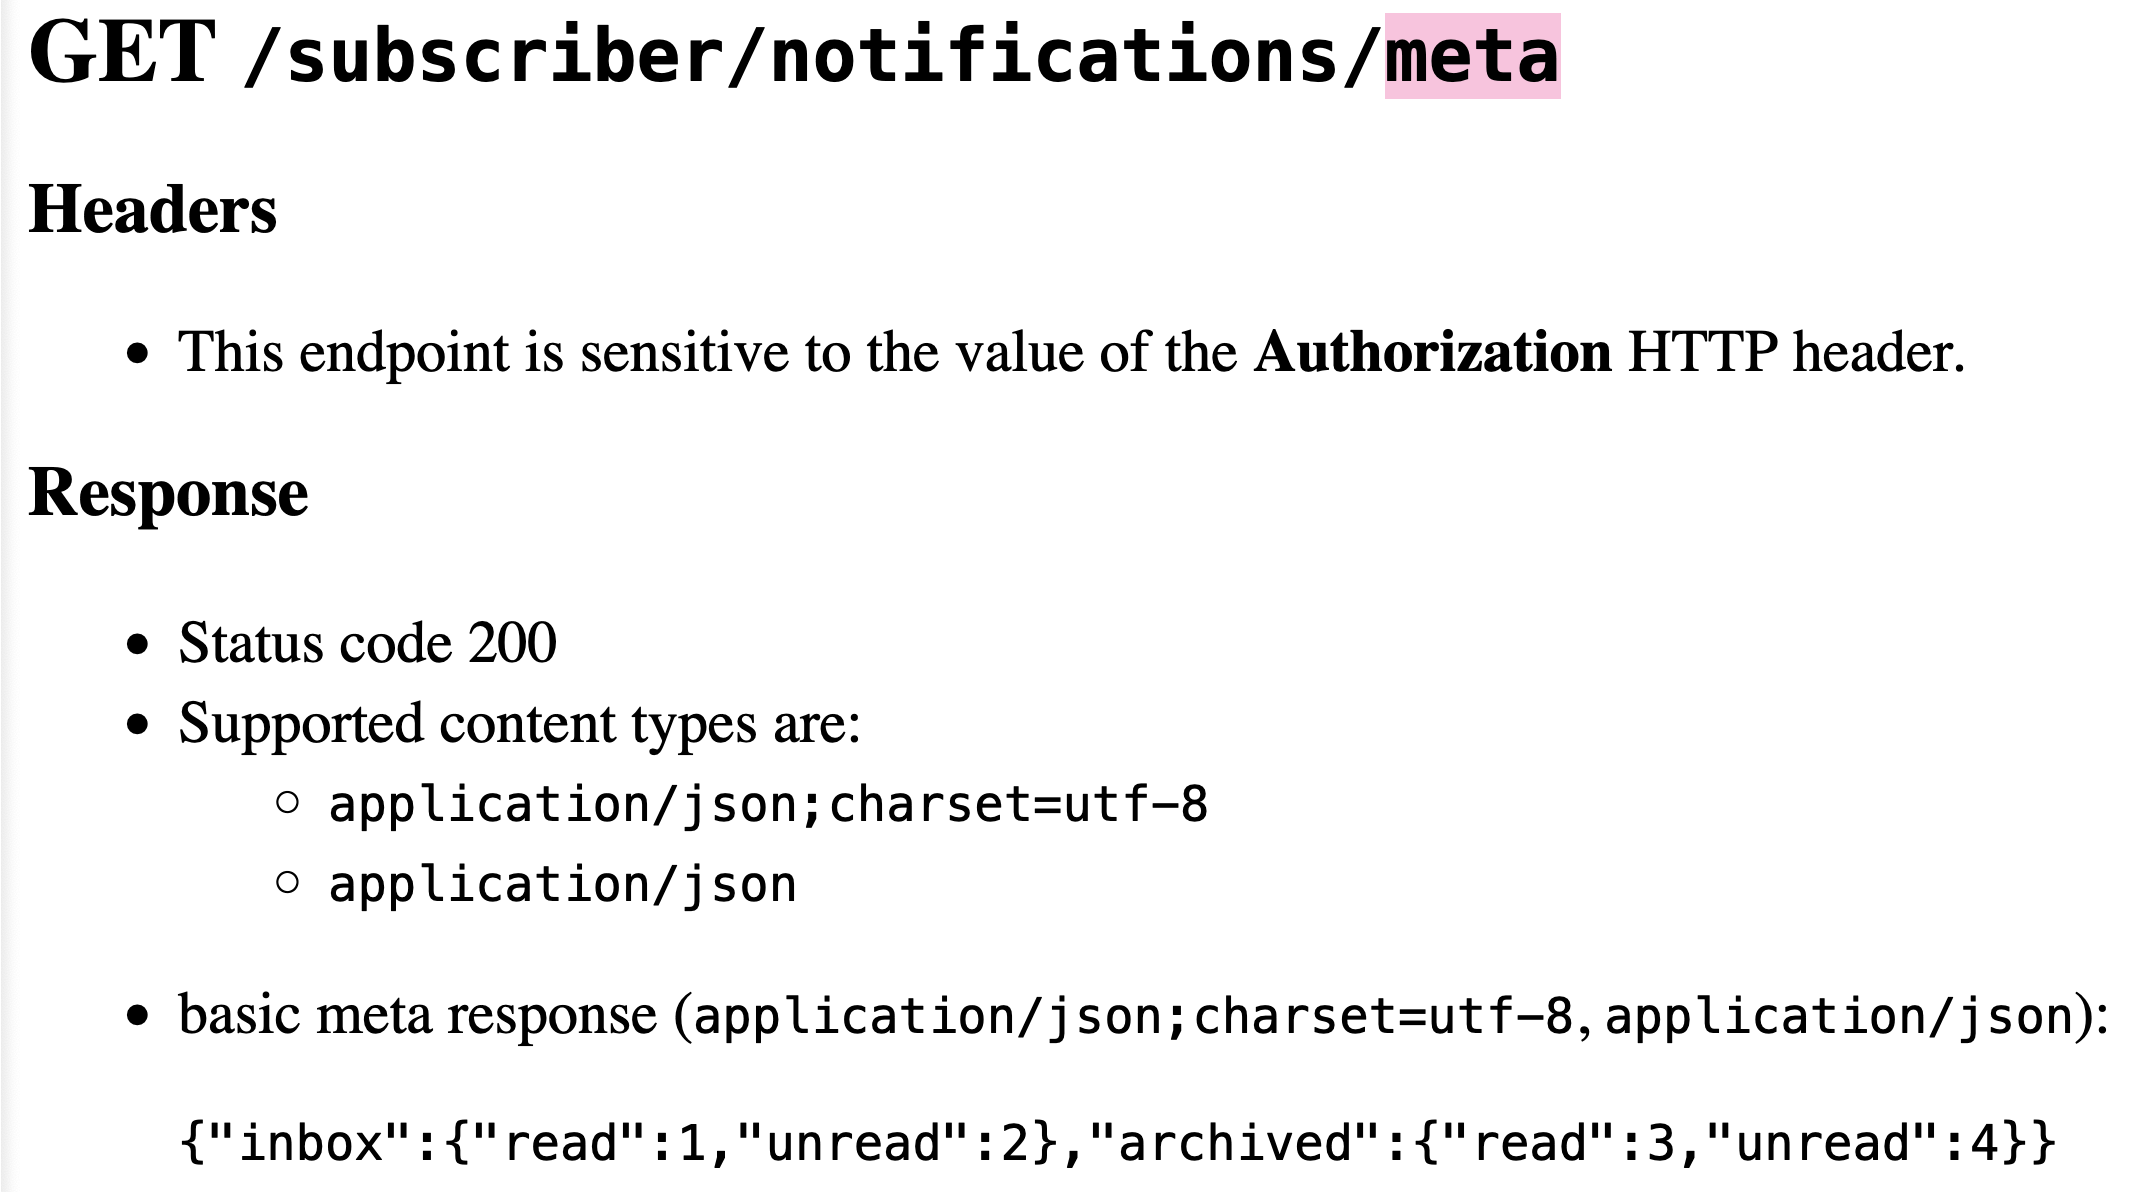
\includegraphics[height=.6\textheight]{images/servant.docs.png}
		\caption{
			The type-level encoding can be recursed over to generate
			documentation.
		}
	\end{figure}
\end{frame}

\begin{frame}[fragile]{Even more type-level payoff}
	We can also generate TypeScript code for interopt.
	\begin{block}{Generated ``SimJSON'' TypeScript}
		\begin{minted}{typescript}
export type MetaResponse = {
  inbox: MetaResponseCount
  archived: MetaResponseCount
}

export type MetaResponseCount = {
  read: number
  unread: number
}
        \end{minted}
	\end{block}
\end{frame}

\section{Synthesis: Plain Old Haskell Type Classes}

\begin{frame}[fragile]{Real-world generality}
	\begin{block}{}
		\begin{minted}{haskell}
data Timewise a = Timewise
  { atBeginningOfTime :: a
  , changes :: Map PostgresUTCTime a
  }
  deriving (Eq, Foldable, Functor, Generic, Show, Traversable)
        \end{minted}
	\end{block}
	\begin{block}{}
		\begin{minted}{haskell}
instance Applicative Timewise where
  pure a = Timewise a Map.empty
  (<*>) :: Timewise (a -> b) -> Timewise a -> Timewise b = ...
        \end{minted}
	\end{block}
	\begin{exampleblock}{}
		Typeclasses are great DSLs.
	\end{exampleblock}
\end{frame}

\section{Industry's Brand}

\begin{frame}{Industry's Brand}
	\begin{columns}
		\column{.5\textwidth}
		\begin{itemize}
			\item<1-> ``Nobody got fired for buying IBM.''
			\item<2-> ``Nobody got fired for choosing Java.''
		\end{itemize}
		\column{.5\textwidth}
		\begin{exampleblock}<3->{}
			Remember that most problems Haskell has are common in all languages:
			\begin{itemize}
				\item resilience
				\item deployment
				\item observability
				\item testing (modularity).
			\end{itemize}
		\end{exampleblock}
		\begin{exampleblock}<3->{}
			Empathize with the perspective of non-Haskellers.
		\end{exampleblock}
	\end{columns}
\end{frame}

\begin{frame}{SimSpace's Growth}
	\begin{columns}
		\column{.5\textwidth}
		Adoption of FP and Haskell wasn't hard
		\begin{itemize}
			\item Reasonable people
			\item Lots of trust
		\end{itemize}
		Our challenges happened as we grew.
		\column{.5\textwidth}
		\begin{exampleblock}<2->{}
			Value expertise.
		\end{exampleblock}
		\begin{exampleblock}<2->{}
			Have a preferred way of doing things.
			\begin{itemize}
					\item libraries/services and integration
					\item testing strategies
			\end{itemize}
		\end{exampleblock}
		\begin{exampleblock}<2->{}
			Balance internal standards with innovation.
		\end{exampleblock}
	\end{columns}
\end{frame}

\begin{frame}{Compilation time woes}
	\begin{columns}
		\column{.5\textwidth}
		\begin{itemize}
			\item Compilation times slowly got worse
			\item It's easy to get inured
			\item Productivity lost between CI and rebasing
			\item Non-Haskellers noticed
			\item Caching with Nix cut development cycle in half
			\item Still work to go
		\end{itemize}
		\column{.5\textwidth}
		\begin{exampleblock}<2->{}
			Track trends in build times actively.
		\end{exampleblock}
		\begin{exampleblock}<2->{}
			Value modularity.
		\end{exampleblock}
		\begin{exampleblock}<2->{}
			Watch for bad coupling.
		\end{exampleblock}
	\end{columns}
\end{frame}

\begin{frame}{Question pithy maxims}
	\begin{columns}
		\column{.5\textwidth}
		\begin{alertblock}{Tooling}
		  \begin{itemize}
			\item We don't need a debugger.
			\item We don't need an IDE.
		  \end{itemize}
		\end{alertblock}
		\begin{alertblock}{Learning}
		  \begin{itemize}
			\item You don't need to worry about lazyness.
			\item Evaluation order doesn't matter.
		  \end{itemize}
		\end{alertblock}
		\begin{alertblock}{Compilation}
		  \begin{itemize}
			\item Compilation proves correctness.
			\item The compiler makes refactoring easy.
		  \end{itemize}
		\end{alertblock}
		\column{.5\textwidth}
		\begin{alertblock}{Documentation}
		  \begin{itemize}
			\item Types are the documentation.
			\item Code is self-documenting.
		  \end{itemize}
		\end{alertblock}
		\begin{alertblock}{Abstraction}
		  \begin{itemize}
			\item You Ain't Gonna Need It (YAGNI)
			\item Premature abstraction/optimization
		  \end{itemize}
		\end{alertblock}
	\end{columns}
\end{frame}

\begin{frame}{Make Haskell accessible}
	\begin{columns}
		\column{.5\textwidth}
		\begin{itemize}
			\item There's enough Haskellers out there.
			\item These candidate hires generally
			      \begin{itemize}
				      \item care a \emph{lot} about quality
				      \item care a \emph{lot} about abstraction
				      \item take much initiative
				      \item are peculiarly auto-didactic
			      \end{itemize}
			\item But many rely on \emph{\textbf{\alert{privilege}}} to pick up
			      enough Haskell skills for industry.
		\end{itemize}
		\begin{exampleblock}<2->{}
			Invest in community, mentorship, and entry-level positions.
		\end{exampleblock}
		\column{.5\textwidth}
		\begin{exampleblock}<2->{}
			Have internal training material that
			\begin{itemize}
				\item reduces starting points
				\item explains how things fit together.
			\end{itemize}
		\end{exampleblock}
		\begin{exampleblock}<2->{}
			Have clean example projects.
		\end{exampleblock}
		\begin{exampleblock}<2->{}
			Don't let complexity constrain onboarding.
		\end{exampleblock}
		\begin{exampleblock}<2->{}
			What's good for diversity is good for all.
		\end{exampleblock}
	\end{columns}
\end{frame}

\begin{frame}{Beyond SimSpace}
	\begin{columns}
		\column{.5\textwidth}
		Excited for
		\begin{itemize}
			\item new energy in the Haskell Foundation
			\item Haskell Language Server
			\item GHC and library improvements
			\item Cabal/Stack improvements.
		\end{itemize}
		\column{.5\textwidth}
		Wishing for
		\begin{itemize}
			\item faster compilations
			\item ergonomic story for a distributed build cache
			\item IDE features like code navigation to third-party libraries.
			\item ergonomic stack traces
		\end{itemize}
	\end{columns}
\end{frame}

\begin{frame}{Lastly}
	\begin{exampleblock}{}
		Seriously consider non-technical roles.
	\end{exampleblock}
	\begin{exampleblock}<2->{}
		Have fun!
	\end{exampleblock}
\end{frame}

\section{Thanks! Questions?}

\end{document}
